%1. Grundlagen
\chapter{Grundlagen}
Diese Studienarbeit befasst sich mit dem komplexen Thema der Elliptischen Kurven in der Kryptographie. Die Kryptographie ist ein stark mathematisches Thema, bei welchem es zu Anfang der Legung einer Grundlage für das Verständnis der Inhalte dieser Studienarbeit. In diesem Kapitel werden sowohl die mathematischen als auch die kryptographischen Grundlagen zum Verständnis der in dieser Arbeit behandelten Elliptischen Kurven der Charakteristik p>3 gelegt. \cite[vgl.][S. 10]{it_sicherheit}

\begin{figure}[!h]
\centering
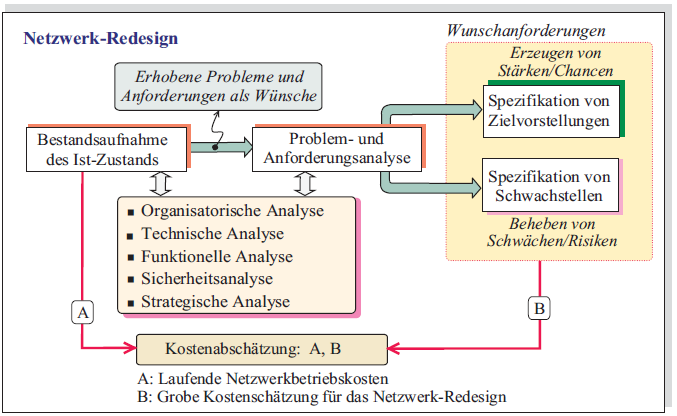
\includegraphics[width=\textwidth]{grafiken/aufgaben_redesign.png}
\caption[Hauptaufgaben der Ist-Analyse beim Redesign einer Netzwerkinfrastruktur]{Hauptaufgaben der Ist-Analyse beim Redesign einer Netzwerkinfrastruktur \\ Quelle: \cite[vgl.][S. 69]{netzwerkprojekte}}
\label{fig:aufgaben_redesign}
\end{figure}

\section{Primzahlen}
XXX

\subsection{Definition}
x

\subsection{Eigenschaften}
x

\subsection{Bestimmung von Primzahlen}
x

\subsection{Rolle der Primzahlen in der Kryptologie}
x

\section{Allgemeines zur Verschlüsselung}
XXX

\subsection{Symmetrische und Asymmetrische Verschlüsselung}
x

\subsection{Diffie-Hellmann}
x

\section{Ziel der Arbeit}
XXX

\section{Geplante Vorgehensweise}
XXX